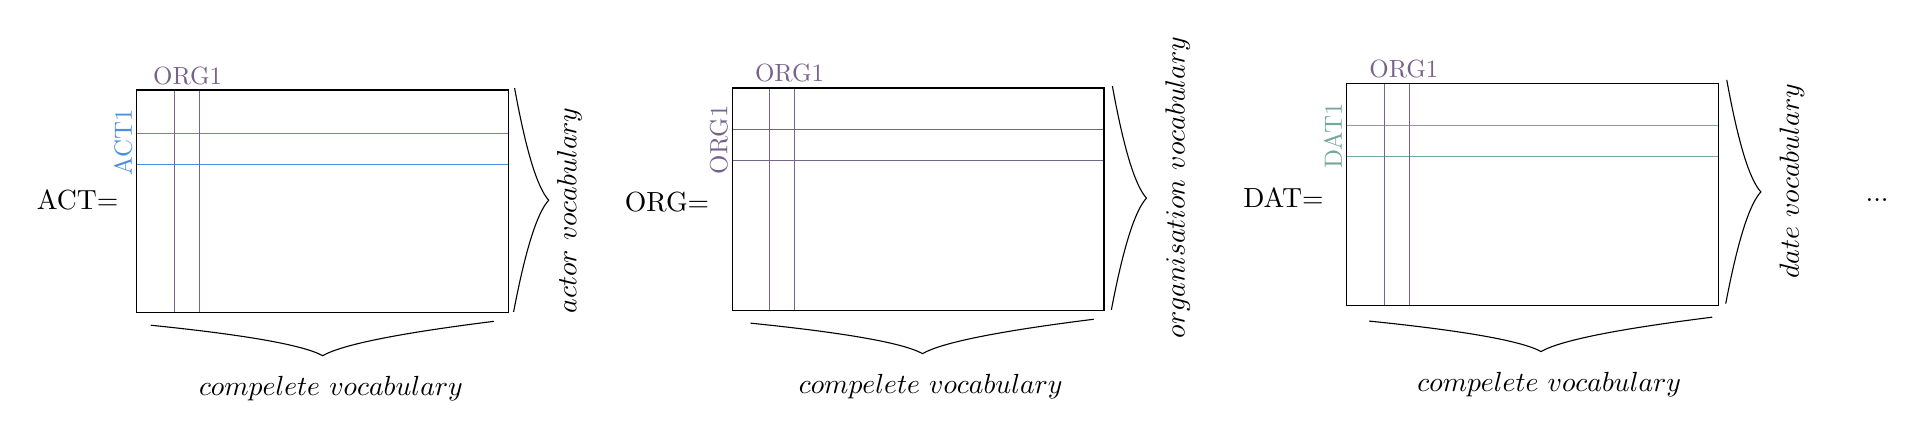
\begin{tikzpicture}[x=0.75pt,y=0.75pt,yscale=-1,xscale=1]
%uncomment if require: \path (0,370); %set diagram left start at 0, and has height of 370

%Shape: Rectangle [id:dp688565454623014] 
\draw  [color={rgb, 255:red, 74; green, 144; blue, 226 }  ,draw opacity=1 ] (55.5,122) -- (234.5,122) -- (234.5,137) -- (55.5,137) -- cycle ;
\draw   (227.55,212.43) .. controls (181.69,218.16) and (154.2,223.68) .. (145.07,228.99) .. controls (135.83,223.89) and (108.22,218.99) .. (62.24,214.31) ;
\draw   (237.54,100.09) .. controls (242.97,130.06) and (248.44,148.05) .. (253.97,154.07) .. controls (248.39,160.03) and (242.75,177.97) .. (237.05,207.89) ;
%Shape: Rectangle [id:dp37213328100124254] 
\draw  [color={rgb, 255:red, 120; green, 99; blue, 139 }  ,draw opacity=1 ] (73.5,101) -- (85.5,101) -- (85.5,208) -- (73.5,208) -- cycle ;
%Shape: Rectangle [id:dp4064945973146499] 
\draw  [color={rgb, 255:red, 0; green, 0; blue, 0 }  ,draw opacity=1 ] (55.5,101) -- (234.5,101) -- (234.5,208) -- (55.5,208) -- cycle ;
%Shape: Rectangle [id:dp5929123930060234] 
\draw  [color={rgb, 255:red, 120; green, 99; blue, 139 }  ,draw opacity=1 ] (342.5,120) -- (521.5,120) -- (521.5,135) -- (342.5,135) -- cycle ;
%Shape: Rectangle [id:dp5111732488988676] 
\draw  [color={rgb, 255:red, 120; green, 99; blue, 139 }  ,draw opacity=1 ] (360.5,100) -- (372.5,100) -- (372.5,207) -- (360.5,207) -- cycle ;
%Shape: Rectangle [id:dp03627212507715449] 
\draw  [color={rgb, 255:red, 0; green, 0; blue, 0 }  ,draw opacity=1 ] (342.5,100) -- (521.5,100) -- (521.5,207) -- (342.5,207) -- cycle ;
%Shape: Rectangle [id:dp8482224250536965] 
\draw  [color={rgb, 255:red, 117; green, 167; blue, 159 }  ,draw opacity=1 ] (638.5,118) -- (817.5,118) -- (817.5,133) -- (638.5,133) -- cycle ;
%Shape: Rectangle [id:dp9261416839296721] 
\draw  [color={rgb, 255:red, 120; green, 99; blue, 139 }  ,draw opacity=1 ] (656.5,98) -- (668.5,98) -- (668.5,205) -- (656.5,205) -- cycle ;
%Shape: Rectangle [id:dp8074449392219452] 
\draw  [color={rgb, 255:red, 0; green, 0; blue, 0 }  ,draw opacity=1 ] (638.5,98) -- (817.5,98) -- (817.5,205) -- (638.5,205) -- cycle ;
\draw   (516.55,211.43) .. controls (470.69,217.16) and (443.2,222.68) .. (434.07,227.99) .. controls (424.83,222.89) and (397.22,217.99) .. (351.24,213.31) ;
\draw   (814.55,210.43) .. controls (768.69,216.16) and (741.2,221.68) .. (732.07,226.99) .. controls (722.83,221.89) and (695.22,216.99) .. (649.24,212.31) ;
\draw   (525.54,99.09) .. controls (530.97,129.06) and (536.44,147.05) .. (541.97,153.07) .. controls (536.39,159.03) and (530.75,176.97) .. (525.05,206.89) ;
\draw   (821.54,96.09) .. controls (826.97,126.06) and (832.44,144.05) .. (837.97,150.07) .. controls (832.39,156.03) and (826.75,173.97) .. (821.05,203.89) ;

% Text Node
\draw (80,94) node [scale=0.9,color={rgb, 255:red, 120; green, 99; blue, 139 }  ,opacity=1 ] [align=left] {ORG1};
% Text Node
\draw (149,245) node   {$compelete\ vocabulary$};
% Text Node
\draw (264,159) node [rotate=-270]  {$actor\ vocabulary$};
% Text Node
\draw (49,126) node [scale=0.9,color={rgb, 255:red, 74; green, 144; blue, 226 }  ,opacity=1 ,rotate=-270] [align=left] {ACT1};
% Text Node
\draw (370,93) node [scale=0.9,color={rgb, 255:red, 120; green, 99; blue, 139 }  ,opacity=1 ] [align=left] {ORG1};
% Text Node
\draw (557,148) node [rotate=-270]  {$organisation\ vocabulary$};
% Text Node
\draw (336,125) node [scale=0.9,color={rgb, 255:red, 120; green, 99; blue, 139 }  ,opacity=1 ,rotate=-270] [align=left] {ORG1};
% Text Node
\draw (666,91) node [scale=0.9,color={rgb, 255:red, 120; green, 99; blue, 139 }  ,opacity=1 ] [align=left] {ORG1};
% Text Node
\draw (853,145) node [rotate=-270]  {$date\ vocabulary$};
% Text Node
\draw (632,123) node [scale=0.9,color={rgb, 255:red, 117; green, 167; blue, 159 }  ,opacity=1 ,rotate=-270] [align=left] {DAT1};
% Text Node
\draw (894,154) node   {$...$};
% Text Node
\draw (27,154) node  [align=left] {ACT=};
% Text Node
\draw (311,155) node  [align=left] {ORG=};
% Text Node
\draw (608,153) node  [align=left] {DAT=};
% Text Node
\draw (438,244) node   {$compelete\ vocabulary$};
% Text Node
\draw (736,243) node   {$compelete\ vocabulary$};


\end{tikzpicture}
